\subsection{Расчет скоростей нейтронного захвата с помощью TALYS}
\subsubsection{Формула астрофизической скорости реакции}
Скорость ядерной реакции $\lambda$ рассчитывается путем свертки ее сечения с энергетическим распределением взаимодействующих частиц. Энергии нейтронов и ядер в звездном веществе имеют распределение Максвелла-Больцмана. Следует учитывать, что при астрофизических температурах ядра находятся в возбужденных состояниях, и в условиях термодинамического равновесия заселенность уровней также должна подчиняться статистике Максвелла-Больцмана. Тем самым формула для астрофизической скорости ядерной реакции, являющейся функцией температуры среды $T$, принимает вид
\begin{equation}
\displaystyle
\lambda(T) = \sqrt{\frac{8}{\pi m}} \frac{N_A}{(k T)^{3/2} G(T)} \int_0^\infty \sum_\mu \frac{(2 I^\mu + 1)}{(2 I^0 + 1)} \sigma^\mu(E) E \exp \left( - \frac{E + E_x^\mu}{kT} \right) dE,
\end{equation}
где $E^\mu_x$ и $I^\mu$ --- энергия и спин возбужденного уровня $\mu$, $m$ --- приведенная масса взаимодействующих частиц, $k$ --- постоянная Больцмана, $N_A$ --- число Авогадро, $G(T)$ --- статистическая сумма
\begin{equation}
    \displaystyle
    G(T) = \sum_\mu \frac{(2 I^\mu + 1)}{(2 I^0 + 1)} \exp \left( - \frac{E_x^\mu}{kT} \right)
\end{equation}

Расчет скорости ядерной реакции требует предварительного расчета зависимости ее сечения от энергии взаимодействия $\sigma(E)$. В настоящей работе рассматривается эволюция астрофизической ядерной системы при температурах не более $6$~ГК. Энергии нейтронов при таких условиях достаточно малы, чтобы реакцию $(n,\gamma)$ можно было рассматривать с точки зрения статистической модели. В настоящей работе скорости астрофизических скоростей реакций нейтронного захвата рассчитывались при помощи программы TALYS, позволяющей задавать различные параметры статистической модели, в частности теоретические массы ядер. 

\subsubsection{Расчет скоростей реакций с помощью TALYS}
Для расчета астрофизических скоростей реакции нейтронного захвата нами использовались микро-коллективная модель FRDM2012~\cite{moller2016} и микроскопическая модель HFB-24~\cite{goriely2013}, внесенные в состав пакета TALYS его разработчиками, а также феноменологический метод LMR2021, предсказания которого были переведены нами в формат TALYS. Расчеты скоростей с массовой моделью HFB D1M~\cite{goriely2009}, также включенной в TALYS по умолчанию, не проводились, так как эта модель, как и HFB-24, является реализацией микроскопического метода Хартри-Фока-Боголюбова, отличаясь лишь использованием потенциала Гоньи вместо потенциала Скирма. В пакет TALYS также внесена таблица экспериментальных масс, построенная на основе базы данных AME2003~\cite{wapstra2003}. Наконец, если при расчете TALYS требуются значения масс, отсутствующие в экспериментальной или заданной теоретической таблице, то программа использует аналитическую формулу Дуфло-Цукера~\cite{duflo1995}.

Для каждой рассматриваемой массовой таблицы нами были проведены расчеты скоростей нейтронного захвата на всех содержащихся в ней изотопах. В случае наличия экспериментальных значений масс AME2003 предпочтение отдавалось им. При отсутствии экспериментального или теоретического значения массы конечного ядра оно вычислялось при помощи формулы Дуфло-Цукера. 

Добавим, что в исходный код программы TALYS нами было внесено изменение, делающее сетку температур, по которой производится расчет астрофизических скоростей, равномерной и более густой. Эта правка никак не влияет на работу статистической модели ядерных реакций, лишь делает выходные данные более подробными ценой некоторого увеличения времени расчета. Все расчеты TALYS, использовавшиеся в настоящей работе, получены на этой измененной версии программы.  

% Пример расчета скоростей и, возможно, сразу и сечений

\subsubsection{Нейтронный захват за границей существования ядер}
Во всех рассмотренных нами массовых таблицах присутствуют изотопы, находящиеся за областью существования ядер, то есть имеющие отрицательные энергии отделения протона $B_p$ или нейтрона $B_n$:
\begin{equation}\begin{aligned}\label{eq:driplines}
B_p(A,Z) &= E_{\text{св}}(A,Z) - E_{\text{св}}(A-1,Z-1),\\
B_n(A,Z) &= E_{\text{св}}(A,Z) - E_{\text{св}}(A-1,Z),
\end{aligned}\end{equation}
где $E_{\text{св}}$ --- энергия связи ядра, зависящая от выбора массовой модели. При отрицательных значениях $B_p$ или $B_n$ ядро фактически не существует. 

Мы провели расчеты скоростей нейтронного захвата в том числе и на этих несуществующих ядрах, чтобы убедиться, что их учет при моделировании $r$-процесса не будет приводить к некорректным результатам. На рис.~\ref{fig:rates_vs_A_tb} представлены зависимости теоретических скоростей реакции $(n,\gamma)$ при $T = 3$~ГК на нейтроноизбыточных изотопах тербия, а также энергии отделения нейтрона $B_n$ для тех же ядер, рассчитанные по данным рассматриваемых нами массовых моделей. Как видно, начиная с массового числа $192$ для некоторых, в первую очередь нечетно-нечетных изотопов $B_n$ резко падает, доходя до отрицательных значений. При этом начинаются сильные колебания скорости $(n,\gamma)$: если конечное ядро имеет отрицательную $B_n$, то и скорость реакции снижается на порядки. 

Таким образом включение реакций $(n,\gamma)$ с образованием несвязанных нейтроноизбыточных ядер в симуляцию $r$-процесса не должно существенно повлиять на результаты моделирования. С другой стороны, учет таких реакций оставляет модели $r$-процесса возможность для некоторой инерции за границы существования. Путь $r$-процесса будет не просто упираться в линию отделения нейтрона из-за отсутствия возможности продвинуться дальше, а естественным образом замедляться.  

\begin{figure}
  \centering
  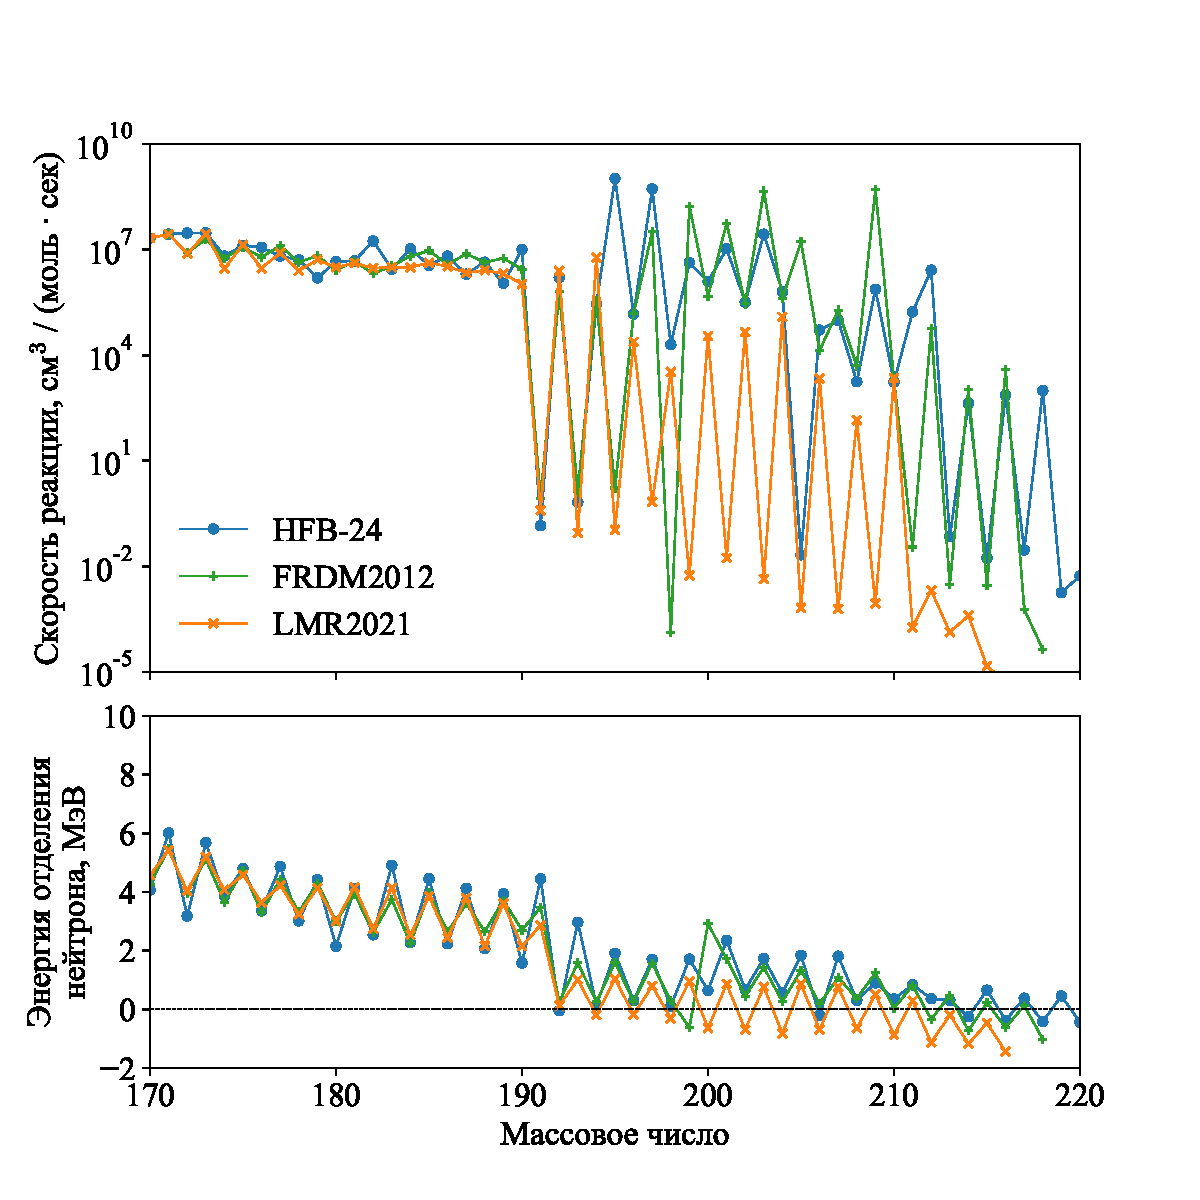
\includegraphics[width=0.6\textwidth]{pics/rates_vs_A_tb.pdf}
  \caption{Свреху: скорости нейтронных захватов на нейтроноизбыточных изотопах тербия, рассчитанные с помощью различных таблиц ядерных масс при $T = 3$~ГК. Снизу: энергии отделения нейтронов для нейтроноизбыточных изотопов тербия по данным тех же массовых таблиц.}
  \label{fig:rates_vs_A}
\end{figure}

